\subsection{Access Modifiers}
\textit{Write code to show how access modifiers work: private, protected, and public, talk about why you would use each of these.}

Sometimes we don't want all the methods and fields in a class to be accessible to everyone. In Java we can restrict access to parts of the class with access modifiers. There are four access modifiers in Java; public, private, protected, and none (default access).

We first create a class with a fields and methods with all four access modifiers.
\begin{lstlisting}[language=Java]
public String publicField = "public field";
private String privateField = "private field";
protected String protectedField = "protected field";
String defaultField = "default field";

public String publicMethod() {
  return "Public Method";
}

private String privateMethod() {
  return "Private Method";
}

protected String protectedMethod() {
  return "Protected Method";
}

String defaultMethod() {
  return "Default Method";
}
\end{lstlisting}

The source for the \texttt{SomeClass.java} class can be found in Appendix K on page \pageref{App:AppendixK}.

We will test whether different classes can access the fields and methods in the \texttt{SomeClass}. We will also see if \texttt{SomeClass} can access the \texttt{InnerClass} members. Figure \ref{fig:accessmodifiers} depicts the setup.

\begin{figure}[!h]\centering % Using \begin{figure*} makes the figure take up the entire width of the page
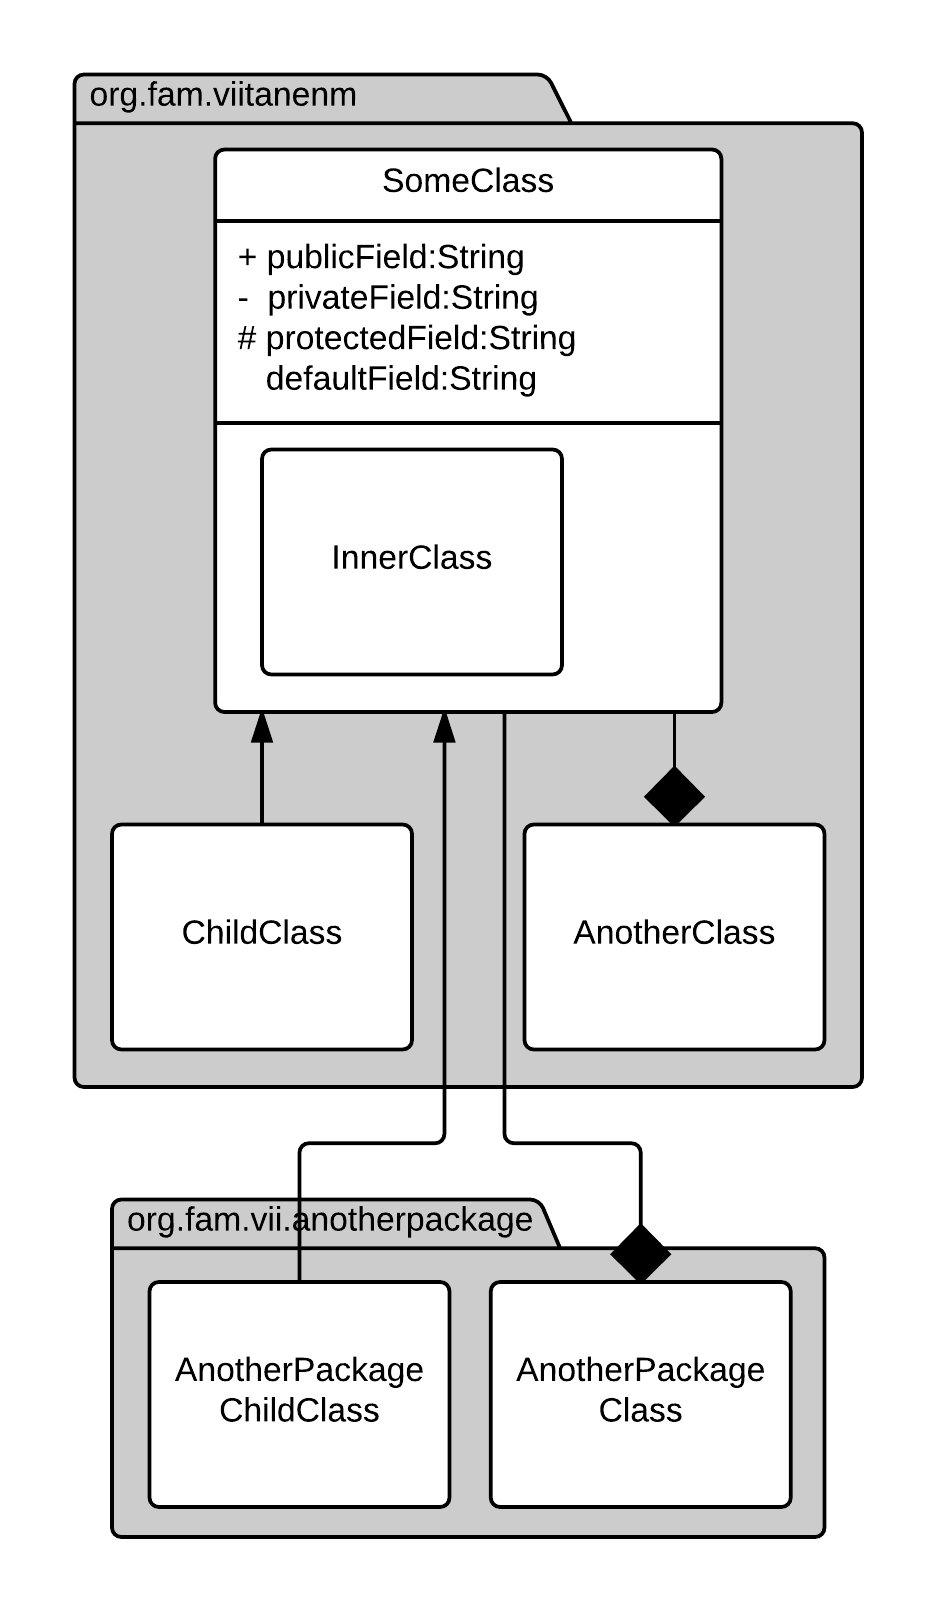
\includegraphics[width=0.9\linewidth, frame]{images/accessmodifiers}
\caption{Composition (Access Modifier Setup)}
\label{fig:accessmodifiers}
\end{figure}

We create an inner class, a class in the same package, a child class, a class in a different package, and a child class in a different package. They all will access the fields and methods in the main class. See the source code for \texttt{AccessModifierExample.java} in Appendix K on page \pageref{App:AppendixK}.

The different classes can access the main classes members as depicted in table \ref{tab:accessmodifiers}.
\setlength{\tabcolsep}{5pt}
\begingroup
\noindent
\def\arraystretch{1.5}
\begin{table}[!htb]
\centering
\begin{tabulary}{\columnwidth}{ | p{0.55\columnwidth} | p{0.05\columnwidth} | p{0.05\columnwidth} | p{0.05\columnwidth}|p{0.05\columnwidth}|} 
\rot{\textbf{}} & \rot{\textbf{public}} & \rot{\textbf{private}}& \rot{\textbf{protected}} & \rot{\textbf{default}}\\ \hline 
Same class & \ding{51} & \ding{51} & \ding{51} & \ding{51} \\ \hline
Class accessing inner class & \ding{51} & \ding{51} & \ding{51} & \ding{51} \\ \hline
Inner class accessing outer class & \ding{51} & \ding{51} & \ding{51} & \ding{51} \\ \hline
A class in the same package & \ding{51} &  & \ding{51} & \ding{51} \\ \hline
Child class & \ding{51} &  & \ding{51} & \ding{51} \\ \hline
Class in another package & \ding{51} &  &  &  \\ \hline
Child class in another package & \ding{51} &  & \ding{51} &  \\ \hline
\end{tabulary}
\caption{Where Different Access Modifiers are Visible}\label{tab:accessmodifiers}
\end{table}
\endgroup
The full output is included in the \texttt{results.txt} in Appendix K on page \pageref{App:AppendixK}.

Interestingly, a child class (in the same package) and a regular class in the same package have exactly the same access. A child class in a different package does not have the default access.